% =========================================================================
% Section 3 — Methodology (DefectSegAM) — Korean version
% \input fragment: no preamble. Uses \TODO and \argmax defined in main.tex.
% =========================================================================
\section{방법론}
\label{sec:method}

본 절에서는 레이어 단위 powder bed 결함 세그멘테이션 네트워크인
DefectSegAM을 기술한다. DefectSegAM은 다음 세 가지 원칙을 중심으로
설계되었다. (i) 동결된(frozen) 비전 파운데이션 모델 인코더(86\,M
파라미터)를 경량의 학습 가능한 디코더(14.6\,M 파라미터)와 결합하여,
이상 탐지 데이터로부터는 디코더만을 학습한다. (ii) 각 적층 레이어의
용융 직후(post-melting) 뷰와 분말 도포 직후(post-spreading) 뷰를
융합하는 명시적인 이중 이미지 변화 단서(change cue)를 도입한다.
(iii) 대규모 pseudo-label(의사 라벨) 사전학습과 소규모 전문가 주석
레이어 코퍼스에 대한 미세조정을 결합한 2단계 라벨 효율적
(label-efficient) 학습 레시피를 사용한다. 그림~\ref{fig:architecture}는
전체 아키텍처의 개요를 보이며, \S\ref{sec:method-problem}에서 과제와
실험에 사용한 클래스 온톨로지를 정의하고,
\S\ref{sec:method-taxonomy}에서 향후 주석을 위한 외형 기준 결함 분류
체계를 제안하며, \S\ref{sec:method-arch}와
\S\ref{sec:method-training}에서 모델과 학습 절차를 제시하고,
\S\ref{sec:method-imbalance}와 \S\ref{sec:method-inference}에서 클래스
불균형 대응 전략과 추론 파이프라인을 상세히 기술한다.

\begin{figure}[t]
\centering
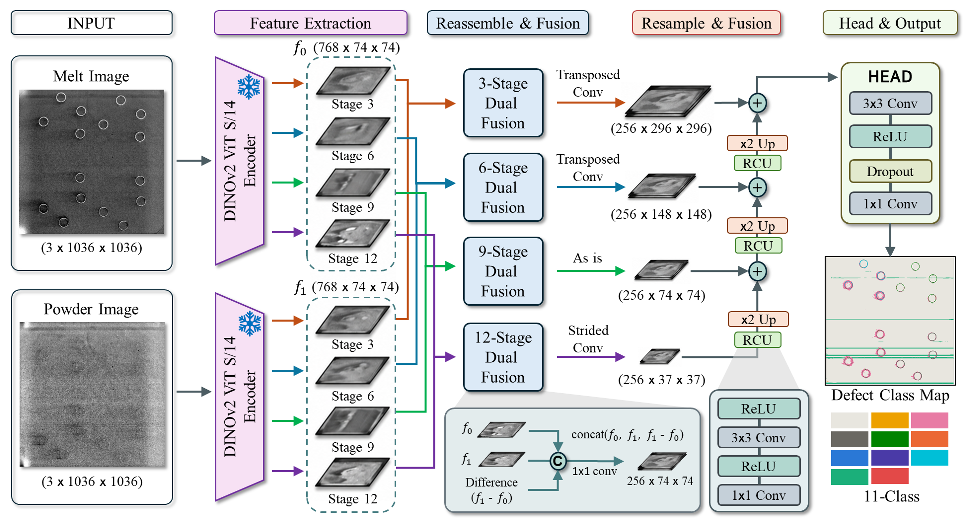
\includegraphics[width=\linewidth]{Figs/DefectSegAM_Architecture.pdf}
\caption{DefectSegAM 아키텍처 개요. 각 레이어의 Melt 이미지 $I_0$와
Powder 이미지 $I_1$은 register token을 포함한 단일 동결 DINOv2
ViT-B/14 인코더(86\,M 파라미터, 가중치 공유 이중 forward)를 통과한다.
트랜스포머 블록 3, 6, 9, 12 이후에서 추출된 특징 맵은 단계별로
$\left[\mathbf{F}^{(0)}_s;\, \mathbf{F}^{(1)}_s;\,
\mathbf{F}^{(1)}_s - \mathbf{F}^{(0)}_s\right]$의
채널 방향 결합(channel-wise concatenation)과 단계별 $1 \times 1$
projection을 통해 256채널로 융합되고, DPT-style reassemble/top-down
융합 디코더(헤드를 포함해 14.6\,M 학습 파라미터)로 디코딩되며,
합성곱 헤드가 산출한 11개 클래스 logit은 bilinear upsampling을 통해
입력 해상도로 복원된다.}
\label{fig:architecture}
\end{figure}

% -------------------------------------------------------------------------
\subsection{문제 설정과 실험용 11-클래스 결함 온톨로지}
\label{sec:method-problem}

Powder bed fusion 공정에서 각 적층 레이어는 두 장의 가시광 카메라
이미지로 기록된다. 하나는 용융(melting) 단계 직후에 촬영되는
\emph{Melt 이미지} $I_0$이고, 다른 하나는 이어지는 분말 도포
(recoating) 단계 이후에 촬영되는 \emph{Powder 이미지} $I_1$이다. 두
뷰는 상호 보완적인 증거를 담고 있으며, DSCNN도 한 레이어의 두 이미지를
함께 입력으로 사용한다~\cite{Scime2020DSCNN}. 개략적으로 정리하면 Recoater
Hopping, Recoater Streaking, Incomplete Spreading, 흩어진 Debris와 같은
도포 관련 이상은 주로 Powder 이미지에서 관찰되는 반면, Spatter, Over
Melting, Under Melting과 같은 용융 관련 이상은 Melt 이미지에 나타나며,
Swelling과 Super-Elevation은 두 이미지 모두에서 드러난다. 이 구분은
저자들의 정리이며, 각 결함이 어느 이미지에서 관찰되는지는
\S\ref{sec:method-taxonomy}에서 외형 기준으로 다시 정리한다. 따라서
DefectSegAM은 이미지 쌍 $(I_0, I_1)$을 입력으로 받아, powder bed의 각
픽셀을 11개 클래스 중 하나에 할당하는 조밀한(dense) 의미 분할(semantic segmentation) 라벨맵
$\hat{M} \in \{0,\dots,10\}^{H \times W}$을 예측한다.

표~\ref{tab:classes}에 정리한 온톨로지는 ORNL Peregrine 플랫폼의
12-클래스 라벨 공간~\cite{Scime2020DSCNN,ORNL_CoRegistered_Dataset}으로부터 유도되며, 이
라벨 공간은 두 개의 비결함 클래스 \emph{Powder}와 \emph{Printed}에 열
개의 이상(anomaly) 클래스를 더한 구성이다. DefectSegAM은 원본 12개
클래스 중 11개를 일대일 매핑으로 유지한다(원본 식별자 0--8은 동일하게
매핑되고, 원본 \emph{Over Melting} 10과 \emph{Under Melting} 11은 각각
9와 10으로 매핑된다). 유일하게 제외되는 클래스는 원본 클래스~9인
\emph{Misprint}(의도된 파트 형상 밖에 프린팅된 재료)이다. Misprint는
베드의 외관이 아니라 CAD 의도를 기준으로 정의되는 클래스이므로,
ignore index $-1$을 할당하여 손실과 모든 평가 지표에서 제외한다.
미세조정 단계에서는 이 온톨로지에 대응 클래스가 없는 다중 장비 GT
코퍼스의 소스 고유(native) 클래스들 역시 동일한 ignore index로
흡수된다(\S\ref{sec:method-training}). 이 온톨로지는 본 논문의 모든
실험이 사용하는 클래스 공간이다. 그 용어가 물려받은 원인 기준과 외형
기준의 혼재, 그리고 이를 정리한 외형 기준 분류 체계는
\S\ref{sec:method-taxonomy}에서 다룬다.

표~\ref{tab:classes}에는 또한 다섯 개의 ORNL 빌드 B1.1--B1.5
전체(Stage-1 학습 \emph{및} 검증; \S\ref{sec:setup}의 필터링된 레이어
집합에 대해 $1036 \times 1036$ 모델 해상도에서 집계)에 대한 재매핑 후
클래스별 총 픽셀 수를 함께 보고한다. 이 분포는 극단적인
long-tail 형태를 보인다. 가장 빈번한 클래스(Powder,
$1.533 \times 10^{10}$ 픽셀)와 가장 희소한 결함 클래스(Recoater
Hopping, 25 픽셀) 사이의 비율은 거의 아홉 자릿수(nine orders of
magnitude)에 이르며, 여러 결함 클래스가 추가로 단일 빌드에 집중되어
있다(예: Over Melting 픽셀의 99.8\,\%와 Under Melting 픽셀의
99.9\,\%는 빌드 B1.2에서, Super-Elevation 픽셀의 98\,\%는 빌드
B1.5에서 발생한다). 이러한 불균형이
\S\ref{sec:method-imbalance}의 샘플링, 증강, 손실 설계의 직접적인
동기가 된다.

\begin{table}[t]
\centering
\caption{DefectSegAM의 11-클래스 온톨로지와 ORNL Peregrine 원본
12-클래스 라벨 공간~\cite{Scime2020DSCNN,ORNL_CoRegistered_Dataset}으로부터의 매핑. 원본
클래스 0--8은 일대일로 매핑되고, 원본 Over Melting(10)과 Under
Melting(11)은 DefectSegAM 식별자 9와 10으로 매핑되며, 유일하게
무시되는 원본 클래스는 Misprint(9)로서 ignore index $-1$에 매핑되어
손실과 평가에서 제외된다. 픽셀 수는 다섯 개의 ORNL Co-Registered 빌드
B1.1--B1.5 전체(\S\ref{sec:setup}의 레이어 필터링을 거친 Stage-1 학습
및 검증 레이어, $1036 \times 1036$ 모델 해상도)에 대한 재매핑 후
총계이다. 설명 열은 ORNL 원 정의를 따른 것이며, 같은 결함을 외형
기준으로 다시 정의한 특징은 표~\ref{tab:taxonomy}에 제시한다.}
\label{tab:classes}
\small
\begin{tabular}{clcp{5.6cm}r}
\toprule
ID & Class & ORNL ID & 설명 & 픽셀 수 (B1.1--B1.5) \\
\midrule
0  & Powder               & 0  & 용융되지 않은 분말 베드 & $1.533 \times 10^{10}$ \\
1  & Printed              & 1  & 용융(프린팅)된 재료 & $7.05 \times 10^{8}$ \\
2  & Recoater Hopping     & 2  & 리코터가 표면 아래의 파트에 부딪혀 발생하는 물결 무늬 & $25$ \\
3  & Recoater Streaking   & 3  & 손상된 리코터 블레이드 또는 끌려간 입자로 인한 줄무늬 & $1.87 \times 10^{8}$ \\
4  & Incomplete Spreading & 4  & 분말 도포량 부족 & $8.67 \times 10^{5}$ \\
5  & Swelling             & 5  & 분말 평면 위로 변형되거나 뒤틀린 프린팅 재료 & $1.0 \times 10^{7}$ \\
6  & Debris               & 6  & 중소 규모 분말 베드 교란을 포괄하는 catch-all 클래스 & $1.8 \times 10^{6}$ \\
7  & Super-Elevation      & 7  & 프린팅 영역 위의 분말 피복 부족 & $2.68 \times 10^{5}$ \\
8  & Spatter              & 8  & 베드 위에 침적된 용융 풀 방출물 & $6.67 \times 10^{8}$ \\
9  & Over Melting         & 10 & 과도한 에너지 밀도로 용융된 영역 & $3.94 \times 10^{5}$ \\
10 & Under Melting        & 11 & 불충분한 에너지 밀도로 용융된 영역 & $2.8 \times 10^{7}$ \\
\midrule
$-1$ (무시됨) & Misprint & 9  & 의도된 파트 형상 밖의 프린팅 재료 & --- \\
\bottomrule
\end{tabular}
\end{table}

% -------------------------------------------------------------------------
\subsection{외형 기준 결함 분류 체계(제안; 실험 미적용)}
\label{sec:method-taxonomy}

표~\ref{tab:classes}의 온톨로지가 물려받은 용어는 판정 기준이 클래스마다
다르다. Over Melting과 Under Melting은 에너지 밀도라는 원인으로,
Misprint는 CAD 의도로 정의되는 반면, 나머지 결함도 상당수는 외형과
원인을 섞어 정의된다. 예컨대 Peregrine v2021-03 릴리스의 정의는
Swelling과 Super-Elevation을 모두 파트가 분말 베드 위로 솟은 외형으로
기술하면서, Swelling은 과도한 국소 에너지 입력, Super-Elevation은 분말
피복 부족 또는 잔류 응력에 의한 뒤틀림의 결과로 원인 절에서만
구분한다~\cite{Peregrine_v2021_03}. 반면 본 논문 라벨의 출처인 ORNL
정의(표~\ref{tab:classes})는 두 클래스를 각각 분말 평면 위로 변형된
프린팅 재료와 프린팅 영역 위의 분말 피복 부족으로 기술하므로, 같은
클래스라도 릴리스마다 판정 기준이 다르다. 저자들의 관찰로는 두 클래스가
이미지에서 모두 파트가 분말 위로 솟은 유사한 형상으로 나타나 구별하기
어렵다. ASTM E3353-22 표준 지침~\cite{ASTME3353}의 공개된 4절도 분말층
이상을 리코팅 오류와 파트 형성 오류라는 원인 범주로 나눌 뿐, skipping과
insufficient powder delivery의 레이어 이미지 외형 차이는 제시하지
않는다(레이어 이미지에서의 상세 기술은 본 연구가 검토하지 못한 8절로
미룬다). 또한 ORNL 12-클래스 공간과 본 연구가 검토한 사람 주석 코퍼스의
클래스 목록에는 둘을 나누는 클래스가 없다. 분말 도포 부족은 L-PBF
소스에서 Incomplete Spreading 하나로만 정의되므로(binder-jet 소스에서는
같은 정의의 Short Feed)~\cite{ORNL_CoRegistered_Dataset,Peregrine_v2021_03,Peregrine_v2022_10},
어느 코퍼스도 둘을 구분하여 주석하지 않는다. 픽셀 단위
주석은 이미지만 보고 수행되므로, 이미지에서 구분할 수 없는 기준은 주석자
간 불일치와 라벨 노이즈로 이어진다. 분말 베드 이미지의 외형으로 이상을
검출·분류한다는 접근 자체는 Scime와 Beuth~\cite{Scime2018Anomaly}와
DSCNN~\cite{Scime2020DSCNN}이 이미 취한 것이지만, 그 클래스 정의는 위와
같이 원인과 CAD 의도를 포함한다. 본 연구는 그 원칙을 명시적 규칙으로
확장한다. 즉 데이터셋 정의에 이미 들어 있는 방향 기준(Recoater
Hopping과 Recoater Streaking을 리코팅 방향에 수직·평행한 줄무늬로
정의~\cite{Peregrine_v2021_03,Peregrine_v2022_10})과 영역 기준(ORNL의
Spatter 정의, v2022-10 릴리스의 ``Spatter on
Powder''~\cite{Peregrine_v2022_10}, 그리고 \S\ref{sec:method-inference}의
후처리 규칙 2)을 판별 규칙으로 정리하고, 원인 또는 CAD 기준으로 정의된
클래스를 재정의하거나 제외하며, 외형이 유사하여 구별하기 어려운 클래스를
통합하여, 결함을 \emph{레이어 이미지에 나타난 특징}을 판정 기준으로
정의하는(위치 판정에는 파트 마스크를 보조로 사용하는) 외형
기준(appearance-based) 결함 분류 체계를 제안한다. 이 체계는 결함 여덟
종에 배경 두 종(Powder, Printed)을 더한 10개 클래스로 구성되며(Under
Melting을 외형 기준으로 재정의하여 유지할 경우 결함 아홉 종이 된다;
아래 (v) 참조), 각 클래스가 관찰되는 이미지(도포 직후의 Powder 이미지
$I_1$, 용융 직후의 Melt 이미지 $I_0$, 또는 둘 다), 이미지에 나타난
특징, 그리고 ORNL 12-클래스 공간 및 ASTM E3353-22 어휘와의 대응을
표~\ref{tab:taxonomy}에 정리하였다. 이미지 열은 저자들의 관찰에 따른
것이다. \TODO{이미지 열의 관찰 근거(검토한 소스·레이어 수)를 명시할
것.}

제안 체계의 결함 클래스 여덟 종의 예시 사진을 여덟 장의 그림에 나누어
보인다. 각 패널 아래에는 클래스명과 원자료의 빌드·레이어 표기를
적었으며, 표기의 M160과 M280은 원자료의 장비 표기를 그대로 옮긴
것이다. 어두운 사진에서도 결함이 보이도록 사진에는 자르기(crop) 외에
화면 전체에 균일한 레벨·감마 조정(levels and gamma adjustment)을
적용하였으며, 그 세부와 표시 방식은 그림~\ref{fig:examples-is-rh}의
캡션에 적었다. 그림~\ref{fig:examples-is-rh}(a)--(c)는 Incomplete
Spreading으로, 분말이 고르게 덮인 영역과 그렇지 않은 영역의 경계(이하
도포 경계)를 점선으로 표시하였다. (a)에서는 도포 경계가 베드 위쪽에서
불규칙하게 내려오고, (b)에서는 왼쪽과 오른쪽에 호 모양의 도포 경계가
하나씩 있으며, (c)에서는 왼쪽에 사선 방향의 도포 경계가 있다. (c)의 흰
상자 두 곳은 원자료가 Over Melting으로 표시한, 표면이 거뭇하게 변색된
파트이다. (d)는 Recoater Hopping으로, 시편 배열의 둘째 행과 셋째 행을
가로질러 가로 띠가 반복된다. 그림~\ref{fig:examples-pc}의 네 장은 같은
빌드에서 촬영된 Powder Collapse이다. 레이어 1323의 (a)에서는 베드
아래쪽 가장자리의 분말이 함몰되어 있고(확대 인셋), 레이어 1455의
(b)에서는 오른쪽 가장자리에 길쭉한 함몰 두 곳이, 레이어 1531의
(c)에서는 오른쪽 가장자리의 함몰과 베드 중앙의 원형 함몰이 보인다.
원자료에 레이어 번호가 없는 (d)에서는 중앙의 함몰이 (c)보다 크고,
오른쪽 가장자리의 함몰도 보인다. 저자들의 관찰로는 이 빌드에서 파트가
움직이면서 분말이 무너졌으며, 파트가 없는 분말을 레이저가 조사하여 생긴
흔적을 Over Melting으로 볼지는 정하지 못하였다. \TODO{(d)의 레이어
번호를 확인하고, 파트 이탈 뒤 분말만 조사된 영역의 클래스(Over Melting
여부)를 확정할 것.}

그림~\ref{fig:examples-rs1} 및
그림~\ref{fig:examples-rs2}의 여덟 장은 Recoater Streaking이다.
그림~\ref{fig:examples-rs1}(a)에는 세로 줄무늬 세 줄이 있다. (b)는
줄무늬가 매우 희미하여, 분말 픽셀의 열 방향 평균 밝기가 주변보다 낮은
두 위치만 표시하였다. (c)에는 분말 위로 드러난 파트를 지나는 굵은 세로
줄무늬 한 줄이 있고, (d)의 줄무늬는 넓은 띠로 발달해 있다(기울어진
상자). 그림~\ref{fig:examples-rs2}(a)는 희미하고 가는 세로 줄무늬
묶음, (b)는 뚜렷한 세로 줄무늬 한 줄과 희미한 한 줄, (c)는 시편을
지나는 세로 줄무늬 세 줄, (d)는 베드 왼쪽에 조밀하게 반복되는 세로
줄무늬이다. 제안 체계의 판별 규칙에서 Recoater Streaking은 리코팅
방향과 평행한 줄무늬, Recoater Hopping은 리코팅 방향과 수직인 반복
줄무늬이지만, 사진의 실제 리코팅 방향은 확인하지 못하였으므로
그림~\ref{fig:examples-rs1} 및 그림~\ref{fig:examples-rs2}의 세로
줄무늬와 그림~\ref{fig:examples-is-rh}(d)의 가로 띠에 대한 클래스
판정은 원자료의 분류에 따른 것이다.

그림~\ref{fig:examples-se1}의 네 장과
그림~\ref{fig:examples-se2-sp}(a)--(c)는 Super Elevation이다.
그림~\ref{fig:examples-se1}(a)에서는 긴 막대형 파트가 분말 위로 드러나
있고, 흰 상자는 원자료가 Over Melting으로 표시한 막대 끝의 밝은
부분이다. (b)에서는 사선 방향 파트의 가장자리 일곱 곳이 분말 위로
드러나 있으며(확대 인셋), 흰 상자는 세로 줄무늬(Recoater
Streaking)이다. (c)에서는 파트 끝이 분말 위로 드러나 있고(확대 인셋),
흰 점선은 도포 경계(Incomplete Spreading)이다. (d)에서는 긴 파트의
가장자리가 솟아 어두운 선으로 보이며, 흰 상자 두 곳은 세로 줄무늬이다.
그림~\ref{fig:examples-se2-sp}(a)에서는 시편 아홉 개의 앞쪽 가장자리가
분말 위로 드러나 있는데(확대 인셋), 저자들은 시편이 반짝이는 것으로
보아 Powder Collapse가 있었을 것으로 추정한다. (b)에서는 빗살 모양
파트의 살 끝이 솟아 변색되어 있다. (c)에는 Super Elevation(시편 세
줄)과 Spatter(시편 왼쪽 분말 영역에 흩어진 검은 입자, 세 곳)가 함께
나타나며, 두 클래스가 모두 이 그림의 대상이므로 둘 다 붉은색으로
표시하고 약어 태그(SE, SP)로 구분하였다. (d)는 Spatter로, 오른쪽 위
시편 세 개의 왼쪽 분말 영역이 어둡게 보인다.

그림~\ref{fig:examples-om}(a)--(c)는 Over Melting이고, (d)는 (c)의
붉은 상자를 확대한 것이다. (a)에서는 고리 모양 파트의 안쪽 표면 두
곳이 거뭇하게 변색되어 있다. (b)에서는 막대형 파트의 표면이 검게
변색되어 있으며(기울어진 상자), 흰 상자는 분말 위로 드러난 파트(Super
Elevation)이다. (c)에서는 $5 \times 5$ 시편 배열의 오른쪽 위 네 시편이
거뭇하게 변색되어 있다. 이와 같이 어둡게 보이는 외형은 외형 기준의
판정 근거일 뿐, 그 자체가 해당 파트의 규격 이탈(out of
specification)을 뜻하지는 않는다.
그림~\ref{fig:examples-db}(a)--(c)는 Debris이고, (d)는 (a)의
확대이다. (a)의 붉은 상자는 분말 면의 검은 덩어리이고, 흰 상자는 분말
위로 드러난 파트(Super Elevation)이다. 저자들의 관찰로는 이 사진에서
Debris와 Super Elevation을 구별하기 어려웠으며, 이는 제안 체계의 판별
규칙이 지닌 한계를 보여 주는 사례이다. (b)와 (c)는 같은 빌드의 레이어
86과 88로, 제자리에서 밀려나 분말 면에 놓인 파트 조각이 각각 두 곳
보인다. (c)의 위쪽에는 리코터가 보이며, 저자들의 관찰로는 밀려난
조각이 끝내 리코터에 걸렸다. 이 체계는 차기 주석과 학습을 위한
제안이며, 본 논문의 모든 학습과 평가는 표~\ref{tab:classes}의 11-클래스
온톨로지로 수행되었다.

\begin{table}[t]
\centering
\caption{제안하는(본 논문의 실험에는 사용하지 않은) 외형 기준 결함 분류
체계(결함 8종 + 배경 2종)와 기존 어휘의 대응. 이미지 열은 결함이 나타나는
이미지를 뜻한다($I_1$ = 분말 도포 직후의 Powder 이미지, $I_0$ = 용융
직후의 Melt 이미지, 둘 다 = 두 이미지 모두). ORNL 열은
표~\ref{tab:classes}의 원본 12-클래스 식별자이고, ASTM 열은 ASTM
E3353-22~\cite{ASTME3353}의 이상 용어를 저자들이 대응시킨 것이며, 괄호
안의 영역 구분은 표준이 아니라 본 체계의 판별 규칙에 따른 것이다.}
\label{tab:taxonomy}
\small
\setlength{\tabcolsep}{4pt}
\begin{tabularx}{\textwidth}{@{}>{\raggedright\arraybackslash}p{2.3cm}c>{\raggedright\arraybackslash}X>{\raggedright\arraybackslash}p{2.2cm}>{\raggedright\arraybackslash}p{2.7cm}@{}}
\toprule
클래스 & 이미지 & 이미지에 나타난 특징 & ORNL 12-클래스 & ASTM E3353-22 \\
\midrule
\multicolumn{5}{@{}l}{\emph{배경}} \\
Powder  & --- & 결함도 파트도 없는 분말 베드 & Powder (0) & --- \\
Printed & --- & 결함이 없는 프린팅 영역 & Printed (1) & --- \\
\multicolumn{5}{@{}l}{\emph{결함}} \\
Incomplete Spreading & $I_1$ & 분말 영역에 남는 얕고 미세한 미도포 자국 & Incomplete Spreading (4) & Skipping; Insufficient powder delivery \\
Powder Collapse      & 둘 다 & 분말이 산사태처럼 무너져 내린 큰 형상 & --- (신규) & Skipping; Insufficient powder delivery \\
Recoater Streaking   & 둘 다 & 리코팅 방향과 평행한 줄무늬 & Recoater Streaking (3) & Scraping \\
Recoater Hopping     & 둘 다 & 리코팅 방향과 수직인 반복 줄무늬 & Recoater Hopping (2) & Part strike \\
Super Elevation      & $I_1$ & 파트가 분말 위로 돌출된 형상 & Swelling (5); Super-Elevation (7) & Distortion; Superelevation; Humping (잠정) \\
Spatter              & $I_0$ & 분말 영역에 재가 날린 것처럼 보이는 거뭇한 영역 & Spatter (8) & Excessive spatter/ejecta (분말 영역) \\
Over Melting         & $I_0$ & 파트 영역 위에 거뭇하게 재가 보이는 영역 & Over Melting (10; 재검토) & Overheating\slash Overmelting; Excessive spatter/ejecta (파트 영역) \\
Debris               & 둘 다 & 분말 면에 포착된 불규칙한 덩어리나 조각 & Debris (6) & --- \\
\midrule
(제외) & --- & CAD 의도 기준 클래스 & Misprint (9) & --- \\
(미결) & --- & 공정 파라미터 기준 클래스; 처리 미결(본문 참조) & Under Melting (11) & --- \\
\bottomrule
\multicolumn{5}{@{}p{\textwidth}@{}}{\footnotesize 이미지 열은 저자들의 관찰에 따른 것으로(Powder
Collapse는 두 코퍼스에 라벨된 사례가 없어 신규 주석 시 확인이 필요하다),
\S\ref{sec:method-problem}의 개략적 구분과는 Swelling/Super-Elevation(둘 다 $\rightarrow$ $I_1$)과
Recoater Streaking, Recoater Hopping, Debris($I_1$ $\rightarrow$ 둘 다)에서 차이가 있다.
특징 열에는 시각 특징만 적었으며, 통상적 원인은 판정 기준이 아니다.
배경 행의 이미지 열 ``---''는 결함이 아니므로 구분이 해당 없음을, 그 밖의 ``---''는 대응 용어가
없음을 뜻한다.
Swelling과 Super-Elevation을 통합한 클래스는 11-클래스 온톨로지의 Super-Elevation과 구별하기
위해 하이픈 없이 Super Elevation으로 표기하고, ASTM 열의 Superelevation은 표준 원문의 철자이다.
표준의 공개된 4절은 humping을 파트 형성 오류로 들면서 과열의 징후로도 들므로, Humping의
Super Elevation 대응은 트랙 융기의 레이어 이미지 외형을 확인하기 전까지 잠정적이다.
Over Melting의 ORNL 라벨 재매핑에는 재검토가 필요하다(본문 참조).}
\end{tabularx}
\end{table}

\begin{figure}[p]
\centering
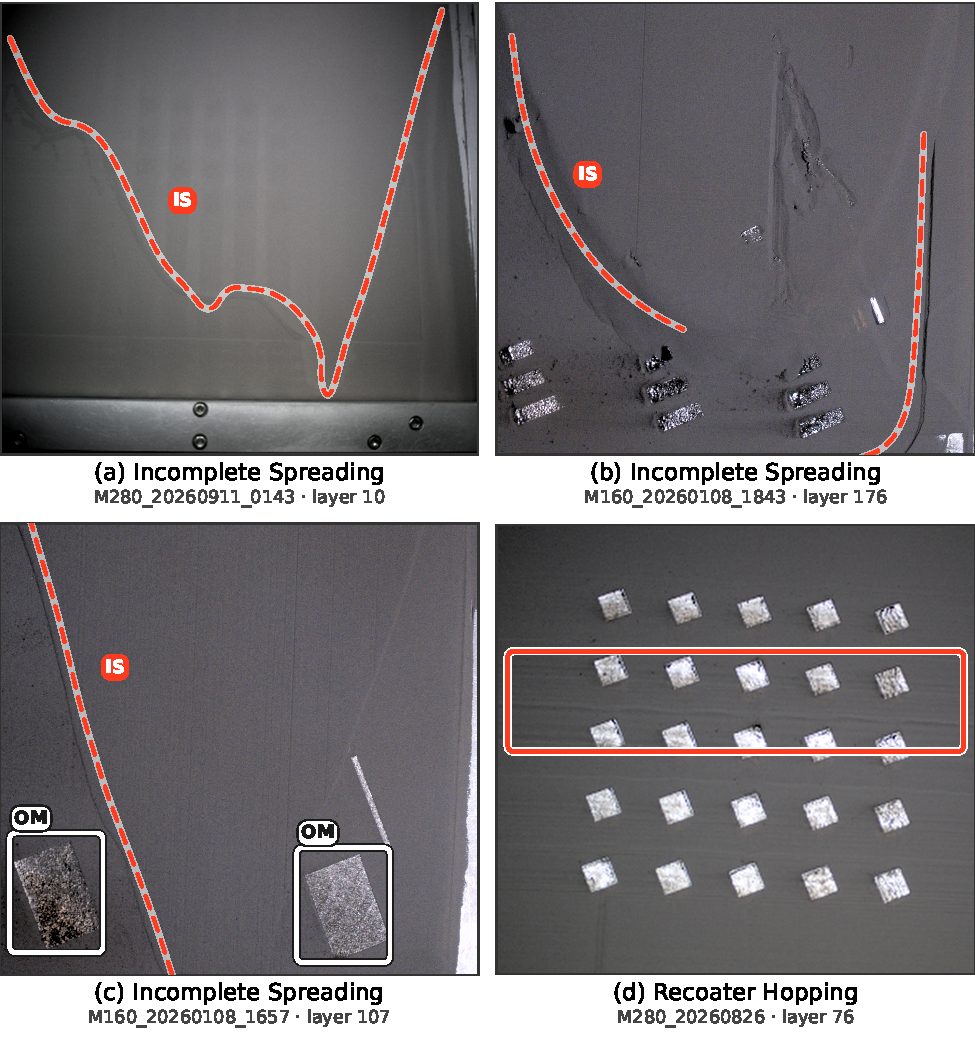
\includegraphics[width=\linewidth,height=0.80\textheight,keepaspectratio]{Figs/Defect_Examples_IS_RH.pdf}
\caption{제안하는 외형 기준 결함 분류 체계(표~\ref{tab:taxonomy})의
예시 사진. (a)--(c) Incomplete Spreading(IS); (d) Recoater Hopping.
저자들이 넣은 표시 중 붉은 것은 해당 그림이 다루는 클래스, 흰 것은
함께 나타난 다른 클래스이고(약어 태그로 구분; OM = Over Melting),
상자는 결함 위치, 점선은 도포 경계 옆에 비켜 그린 안내선, 인셋의
숫자는 확대 배율이다. 사진 처리는 자르기와 사진별로 화면 전체에
균일하게 적용한 레벨·감마 조정뿐이다. 이 조정은 휘도(luminance)
기준이고 선형 증폭은 2.6배 이하, 감마 지수는 0.5--1.0이며, 국소 보정과
합성은 하지 않았다. \TODO{사진의 출처(장비 M160·M280의 정식 명칭,
재료, 카메라)와 사용 허가를 명시할 것.}}
\label{fig:examples-is-rh}
\end{figure}

\begin{figure}[p]
\centering
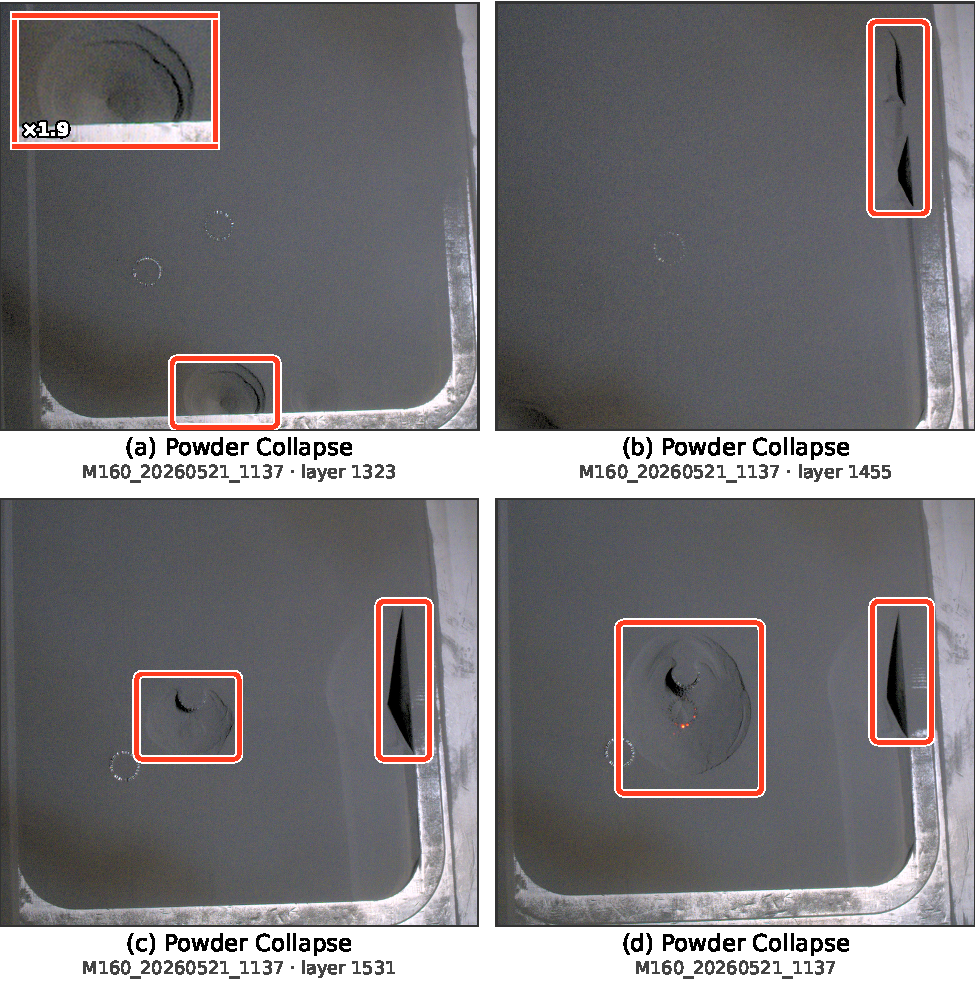
\includegraphics[width=\linewidth,height=0.80\textheight,keepaspectratio]{Figs/Defect_Examples_PC.pdf}
\caption{제안 체계(표~\ref{tab:taxonomy})의 Powder Collapse 예시 사진.
(a)--(d) 같은 빌드에서 촬영된 Powder Collapse. 표시 방식과 사진 처리는
그림~\ref{fig:examples-is-rh}와 같다.}
\label{fig:examples-pc}
\end{figure}

\begin{figure}[p]
\centering
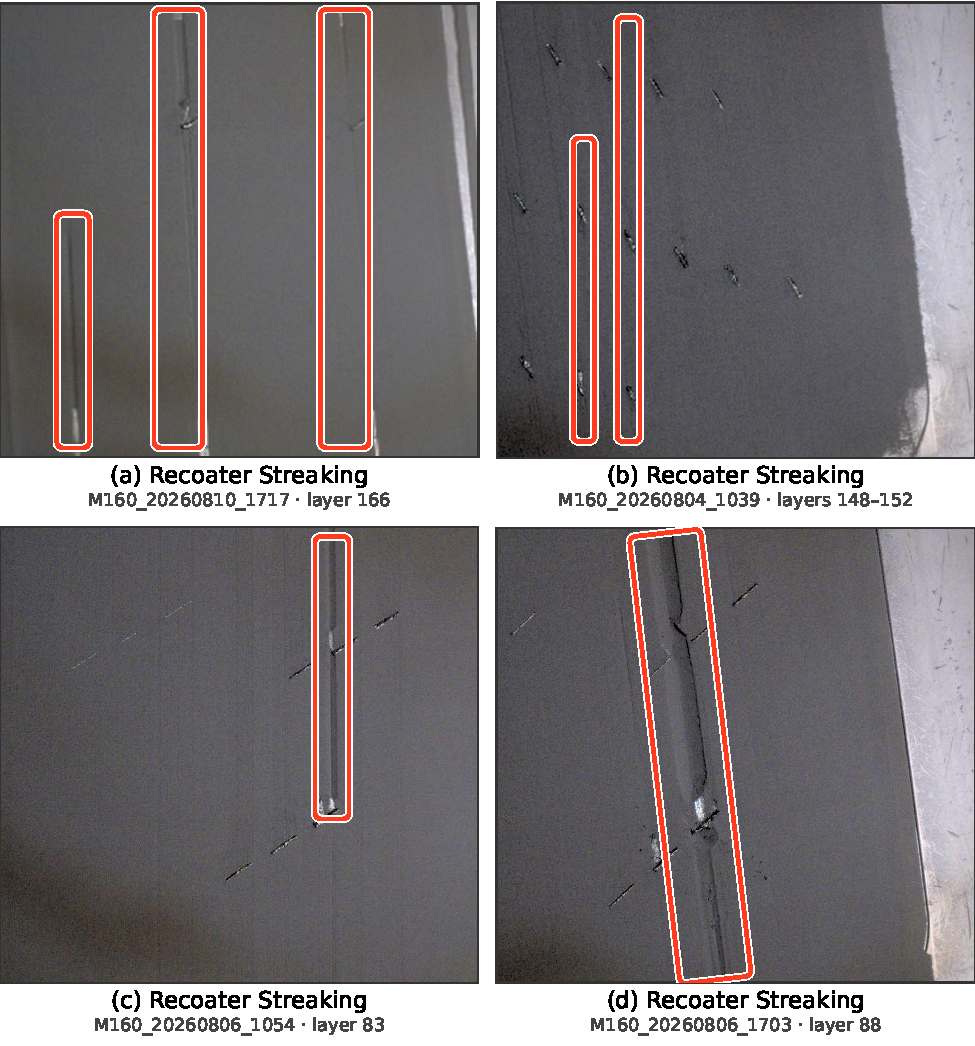
\includegraphics[width=\linewidth,height=0.80\textheight,keepaspectratio]{Figs/Defect_Examples_RS1.pdf}
\caption{제안 체계(표~\ref{tab:taxonomy})의 Recoater Streaking 예시
사진(여덟 장 중 첫 네 장). (a)--(d) Recoater Streaking. 표시 방식과
사진 처리는 그림~\ref{fig:examples-is-rh}와 같다.}
\label{fig:examples-rs1}
\end{figure}

\begin{figure}[p]
\centering
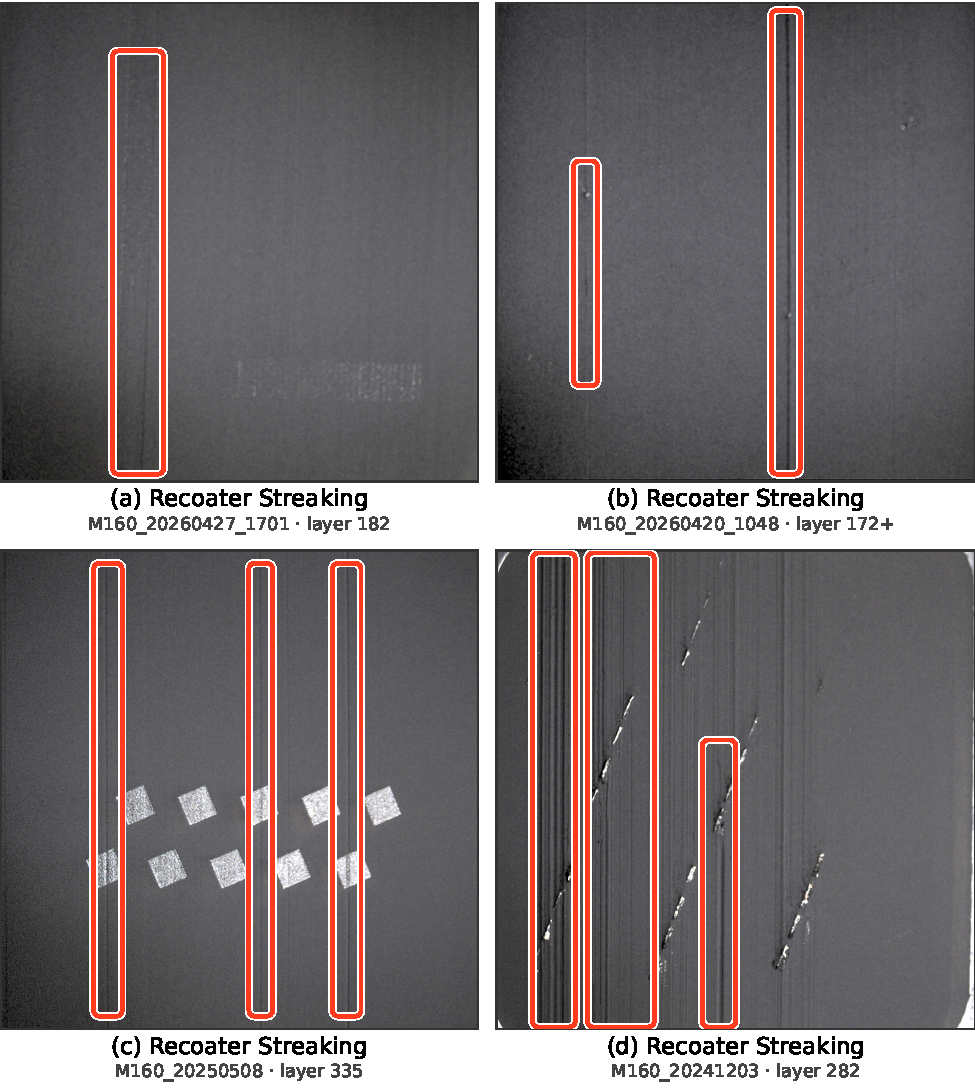
\includegraphics[width=\linewidth,height=0.80\textheight,keepaspectratio]{Figs/Defect_Examples_RS2.pdf}
\caption{제안 체계(표~\ref{tab:taxonomy})의 Recoater Streaking 예시
사진(여덟 장 중 나머지 네 장). (a)--(d) Recoater Streaking. 표시
방식과 사진 처리는 그림~\ref{fig:examples-is-rh}와 같다.}
\label{fig:examples-rs2}
\end{figure}

\begin{figure}[p]
\centering
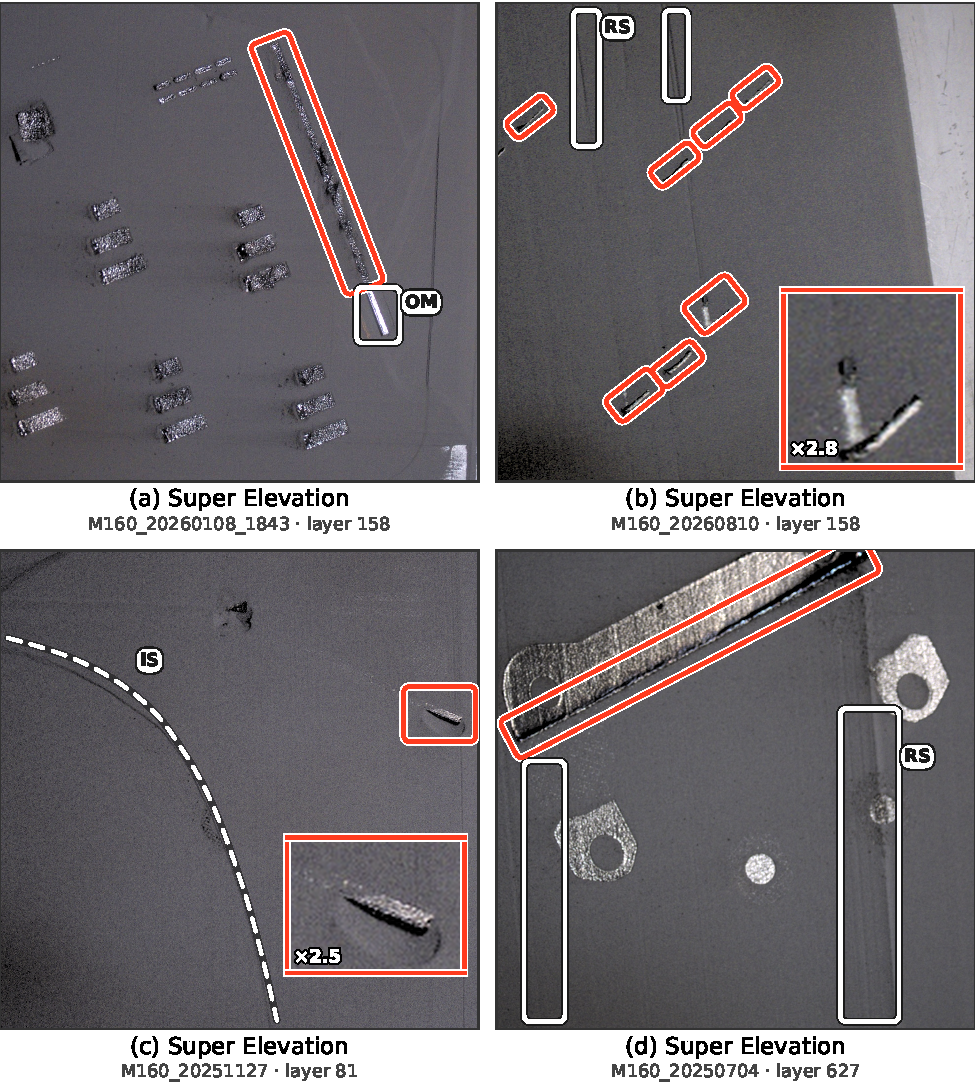
\includegraphics[width=\linewidth,height=0.80\textheight,keepaspectratio]{Figs/Defect_Examples_SE1.pdf}
\caption{제안 체계(표~\ref{tab:taxonomy})의 Super Elevation 예시 사진.
(a)--(d) Super Elevation. 흰 표시는 함께 나타난 Over Melting(OM; (a)),
Recoater Streaking(RS; (b), (d)), Incomplete Spreading(IS; (c)의
점선)이다. 표시 방식과 사진 처리는 그림~\ref{fig:examples-is-rh}와
같다.}
\label{fig:examples-se1}
\end{figure}

\begin{figure}[p]
\centering
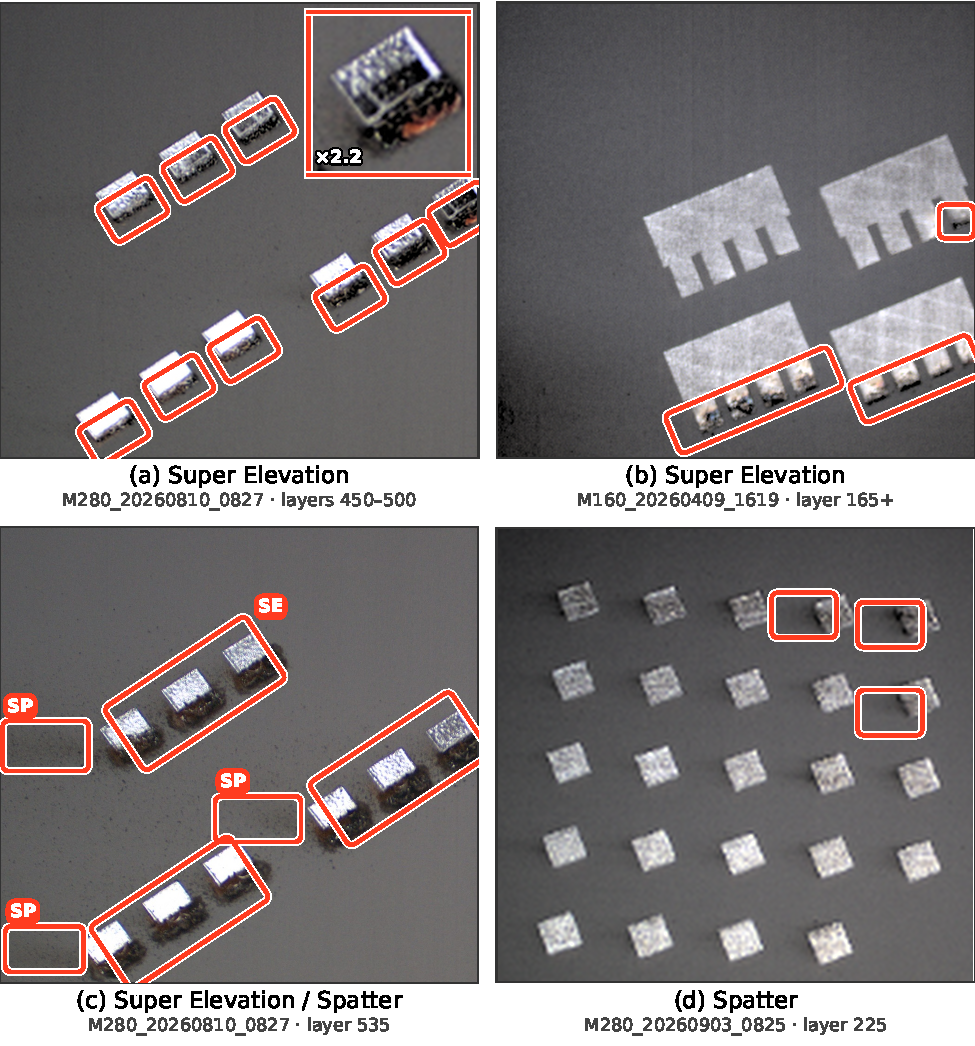
\includegraphics[width=\linewidth,height=0.80\textheight,keepaspectratio]{Figs/Defect_Examples_SE2_SP.pdf}
\caption{제안 체계(표~\ref{tab:taxonomy})의 Super Elevation과 Spatter
예시 사진. (a), (b) Super Elevation; (c) Super Elevation(SE)과
Spatter(SP); (d) Spatter. (c)에서는 두 클래스가 모두 이 그림의
대상이므로 둘 다 붉은색으로 표시하였다. 표시 방식과 사진 처리는
그림~\ref{fig:examples-is-rh}와 같다.}
\label{fig:examples-se2-sp}
\end{figure}

\begin{figure}[p]
\centering
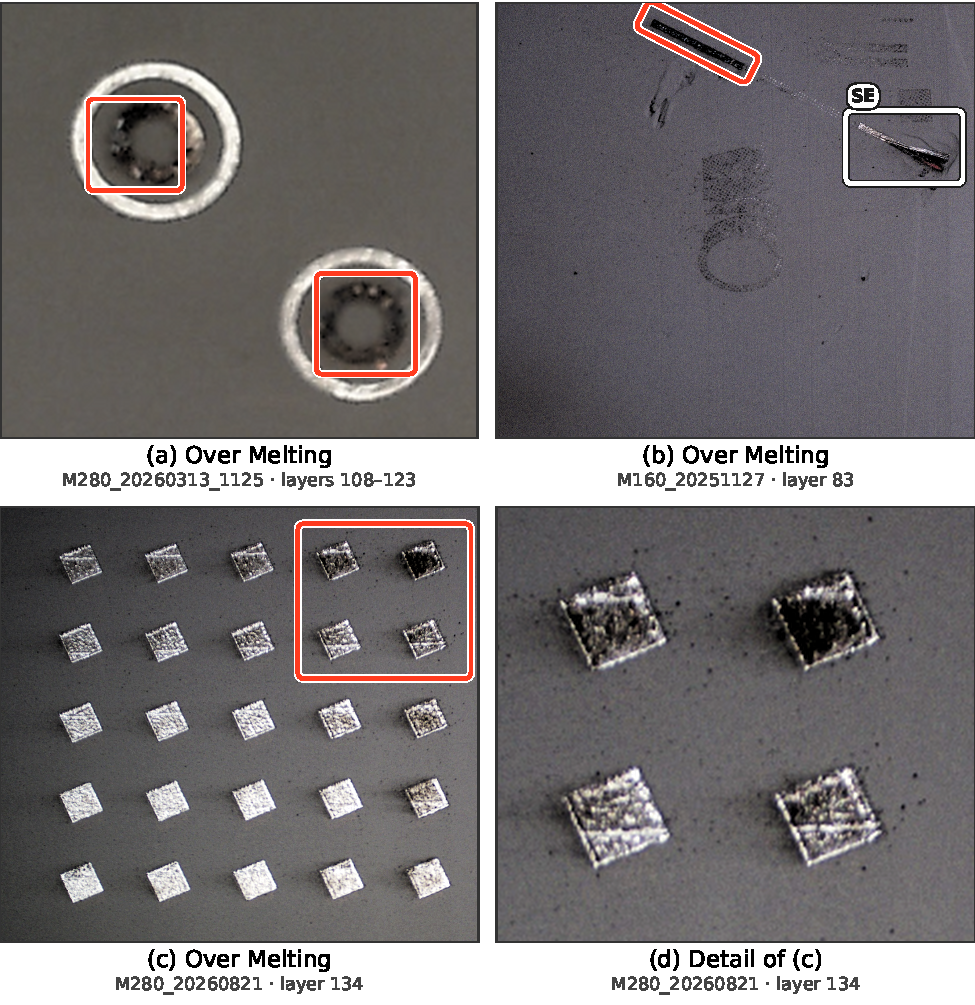
\includegraphics[width=\linewidth,height=0.80\textheight,keepaspectratio]{Figs/Defect_Examples_OM.pdf}
\caption{제안 체계(표~\ref{tab:taxonomy})의 Over Melting 예시 사진.
(a)--(c) Over Melting; (d) (c)의 붉은 상자 영역 확대. (b)의 흰 상자는
함께 나타난 Super Elevation(SE)이다. 표시 방식과 사진 처리는
그림~\ref{fig:examples-is-rh}와 같다.}
\label{fig:examples-om}
\end{figure}

\begin{figure}[p]
\centering
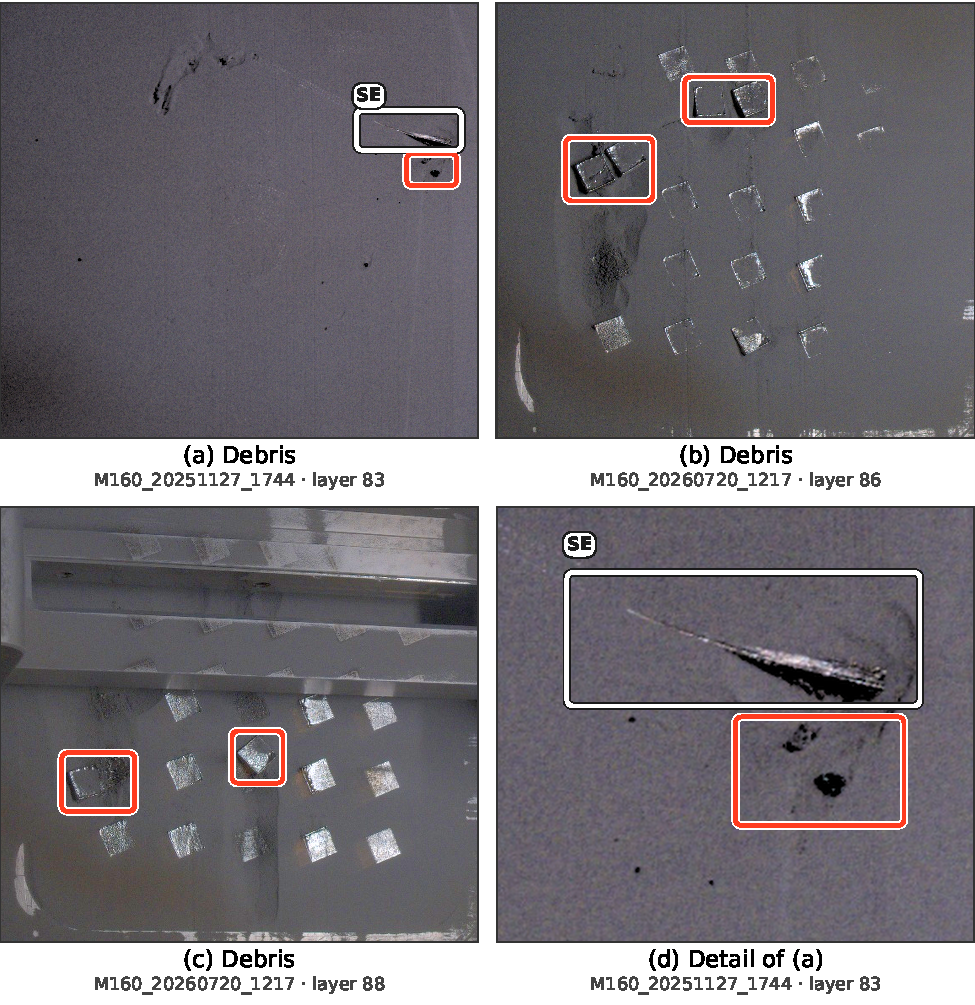
\includegraphics[width=\linewidth,height=0.80\textheight,keepaspectratio]{Figs/Defect_Examples_DB.pdf}
\caption{제안 체계(표~\ref{tab:taxonomy})의 Debris 예시 사진. (a)--(c)
Debris; (d) (a)의 확대. (a)와 (d)의 흰 상자는 함께 나타난 Super
Elevation(SE)이다. 표시 방식과 사진 처리는
그림~\ref{fig:examples-is-rh}와 같다.}
\label{fig:examples-db}
\end{figure}

11-클래스 온톨로지와 비교하면 제안 체계의 변경은 다섯 가지이다. (i)
Swelling과 Super-Elevation은 모두 파트가 분말 위로 솟은 유사한
형상이어서 이미지만으로 구별하기 어려우므로 하나의 Super
Elevation(11-클래스의 Super-Elevation과 구별하기 위해 하이픈 없이
표기한 통합 클래스)으로 통합한다. 면적 기준으로 파트 가장자리의 소규모
융기(Edge Swelling)를 하위 클래스로 분리하는 방안은 임계값을 정한 뒤
검토한다. (ii) 제안 체계는 Spatter와 Over Melting을 모두 거뭇한
영역이라는 외형으로 정의하고(저자들의 관찰로는 두 결함이 유사하게
거뭇하게 나타난다) 위치로만 구분하여, 파트 마스크를 기준으로 분말
영역의 거뭇한 픽셀은 Spatter, 파트 영역의 거뭇한 픽셀은 Over Melting으로
판정한다. 두 클래스를 하나로 합치고 파트 마스크로 후처리 분할하는
대안도 가능하지만, 파트 마스크가 없는 소스(아래 둘째 규칙의 한계)와
실시간 배포에서는 모델이 Printed 영역을 이미지에서 직접 추론해야 하므로
두 클래스를 유지한다. 따라서 두 클래스의 라벨 정의는 파트 마스크에
의존하며, 모델은 파트 영역과 분말 영역의 구분을 이미지에서 학습해야
한다.
(iii) 분말이 무너져 내린 형상은 Incomplete Spreading과 원인(분말
부족)이 일부 겹칠 수 있으나(저자들은 빌드플레이트 패드 마모도 원인으로
추정한다) 이미지 특징이 크게 다르므로 Powder Collapse를 신설한다. (iv)
Misprint는 CAD 의도 기준 클래스이므로 계속 제외한다. 제안 체계도 파트
마스크를 사용하지만, Misprint는 CAD 의도 자체가 판정 기준인 반면 파트
마스크는 위치 정보로만 쓰인다. (v) Under Melting은 저에너지
밀도라는 공정 파라미터로 정의되어 외형 기준 원칙에 어긋난다. Over
Melting을 파트 영역 위의 거뭇한 영역이라는 외형으로 재정의한 것과 달리
Under Melting은 재정의하지 않았다. B1.2에서의 높은 일치도 IoU(0.8643;
\S\ref{sec:results-agreement})는 teacher와 student가 레이어 이미지의
같은 패턴을 이 클래스로 표시함을 뜻하므로 외형 기준 재정의가 가능할 수
있음을 시사하지만, 이는 teacher와의 일치도일 뿐 외형 서명의 존재를 직접
입증하지 않으며(\S\ref{sec:discussion-validity}), 해당 픽셀의
99.9\,\%가 단일 빌드 B1.2에 집중되어 있어 이미지 서명이 그 빌드의 공정
조건과 교락(confounding)되어 있으므로, 주석자가 적용할 수 있는 외형
판정 기준은 아직 정의되지 않았다. ORNL 코퍼스에서 약 $2.8 \times
10^{7}$ 픽셀을 차지하고 본 연구의 11-클래스 온톨로지가 이를 유지하므로,
제안 체계에서의 처리(제외, 또는 외형 기준 재정의와 그 판정 기준)는 향후
과제로 남긴다.
\TODO{제안 체계에서 Under Melting의 처리(ignore 또는 외형 기준 재정의)를
확정할 것; native 클래스 ``Localized Dark Regions''의 Under Melting
매핑(\S\ref{sec:setup})도 함께 결정할 것.}

외형이 비슷한 쌍에는 다음 판별 규칙을 둔다. 첫째, Recoater Streaking과
Recoater Hopping은 줄무늬 방향으로 구분한다. 리코팅 방향과 평행하면
Streaking, 수직이면 Hopping이며, 이 구분은 Peregrine 릴리스의 클래스
정의를 따른 것이다~\cite{Peregrine_v2021_03,Peregrine_v2022_10}. 이
규칙에는 리코팅 방향 메타데이터가 필요하다. Peregrine v2022-10
릴리스~\cite{Peregrine_v2022_10}의 소스 정보 파일과 ORNL Co-Registered
HDF5~\cite{ORNL_CoRegistered_Dataset}의
빌드 메타데이터(\texttt{printer/recoating\_direction}; 다섯 빌드 모두
$-x$)는 리코팅 방향을 기록하므로 이 규칙은 두 코퍼스에 적용할 수 있고,
v2021-03 릴리스~\cite{Peregrine_v2021_03}에는 해당 메타데이터가 없다.
같은 이유로 $90^{\circ}$ 회전은 줄무늬 방향의 의미를 바꾸므로 증강에 쓸
수 없으며, \S\ref{sec:method-inference}의 기하 증강이 flip과
$180^{\circ}$ 회전만 사용하는 것은 이와 부합한다. 둘째, Spatter와 Over
Melting은 파트 마스크로 구분한다. ORNL 데이터셋은 모든 레이어에 파트
식별자 마스크(\texttt{slices/part\_ids})를 제공하므로 이 규칙을 전
레이어에 적용할 수 있다. 반면 Peregrine v2022-10 릴리스의 파트 마스크는
파트 형상 정보가 없는 레이어에서 빈 마스크로 제공된다. 여섯 소스의 학습
분할에 공개된 파트 마스크 88장 중 61장이 빈 마스크이며(17-4~PH와
Inconel~718의 둘째 구성은 전부, maraging steel 소스는 26장 중 15장,
H13은 7장 중 6장, Inconel~718의 첫째 구성은 5장 중 2장), 주석이 있는
85개 레이어(표~\ref{tab:datasets})로 한정해도 61개로 같다. v2021-03
릴리스에는 파트 마스크가 없다. 따라서 사람 주석 코퍼스에서는 이 규칙을
GammaPrint-700 등 파트 마스크가 있는 일부 레이어에만 자동 적용할 수
있고, 나머지 레이어에서는 주석자가 Printed 영역을 직접 판정해야 한다.
셋째,
Incomplete Spreading과 Super Elevation은 둘 다 Powder 이미지에서 분말로
덮이지 않은 형태로 나타나지만, 파트 마스크 안에서 금속 표면이 밝게
드러나면 Super Elevation, 분말 영역에 얕게 덮이다 만 자국이면 Incomplete
Spreading으로 판정한다. 넷째, Incomplete Spreading과 Powder Collapse는
규모와 형상으로 구분한다. 전자는 얕고 미세하며 Powder 이미지에서만
보이지만, 후자는 분말이 무너져 내린 큰 형상이며 용융 뒤에도 남아 Melt
이미지에서도 보일 것으로 예상된다(표~\ref{tab:taxonomy} 각주; 신규 주석
시 확인한다). 이 규칙들에는 다음 한계가 있다. 첫째 규칙은 리코팅
방향 메타데이터가 없는 v2021-03 소스에는 적용할 수 없다. 둘째와 셋째
규칙은 CAD 파트 마스크에 의존하지만, 실제 프린팅 영역은 CAD 형상과
어긋날 수 있고---Misprint와 Super Elevation이 존재하는 이유이기도
하다---마스크 경계에 걸친 픽셀의 처리 규칙이 아직 없다. 또한 둘째와
셋째 규칙은 모두 현재 사람 주석 코퍼스의 대부분 레이어에 자동 적용할 수
없으므로, 마스크가 없거나 빈 레이어에서는 두 규칙 모두 주석자가 파트
영역을 직접 판정해야 한다. 넷째 규칙의
규모 기준에는 정량 임계값이 없다. 이 규칙들이 주석자 간 불일치를 실제로
줄이는지는 측정되지 않았으므로, 재주석 시 복수 주석자의 클래스별
일치도로 검증해야 한다.

제안 체계를 적용하려면 기존 라벨의 재매핑과 일부 신규 주석이 필요하다.
표~\ref{tab:taxonomy}의 대응에 따라 Powder, Printed, Incomplete
Spreading, Recoater Streaking, Recoater Hopping, Debris는 기존 ORNL 의사
라벨과 사람 주석을 그대로 재매핑할 수 있고(다만 Incomplete Spreading
라벨에 Powder Collapse 형상이 섞여 있는지, 그리고 원 정의상
포괄(catch-all) 클래스인 Debris 라벨이 새 정의(불규칙한 덩어리·조각)를
만족하는지는 재검토가 필요하다), Super
Elevation은 Swelling과 Super-Elevation 라벨의 합집합으로 얻는다. 반면
Spatter와 Over Melting은 기존 라벨을 파트 마스크로 다시 나누어야
하며(ORNL 코퍼스는 \texttt{slices/part\_ids}로 가능하다), ORNL의 Over
Melting은 고에너지 밀도 공정 파라미터라는 원인으로 정의된 클래스이고 그
픽셀의 99.8\,\%가 B1.2에 집중되어 있으므로, 파트 영역 위의 거뭇한
외형이라는 새 정의를 만족하는지 레이어별 재검토가 필요하다. Debris는
ORNL 코퍼스에 약 $1.8 \times 10^{6}$ 픽셀, 사람 주석 코퍼스의 여덟 개
소스 중 다섯 개에 존재한다. Powder Collapse에 해당하는 라벨은 ORNL
코퍼스와 사람 주석 코퍼스 어디에도 없어 신규 주석이 필요하다. Recoater
Hopping은 ORNL 코퍼스에 25픽셀뿐이고 사람 주석은 롤러형 리코터를 쓰는
maraging steel 소스에만 있는데, 이 소스의 정의는 ``롤러가 분말 표면에
만드는 물결 모양 세로선''으로 리코터 블레이드와 파트의 접촉을 전제하는
다른 소스의 정의와 원인이 다르므로~\cite{Peregrine_v2022_10},
외형(리코팅 방향과 수직인 반복 줄무늬)이 일치하는지 확인한 뒤
재매핑해야 한다. 한편 \S\ref{sec:method-training}에서 ignore index로
흡수되는 native 클래스 ``Soot''(확산된 어두운 영역)는 파트 마스크로
나누면 Spatter와 Over Melting의 사람 주석으로 재활용할 수 있다. 그러나
Soot 클래스가 정의된 네 소스 중 v2021-03 L-PBF 소스에는 파트 마스크가
없고, v2022-10의 17-4~PH는 공개된 파트 마스크가 모두 빈
마스크이며(Inconel~718 둘째 구성은 Soot 클래스를 정의하지만 주석 픽셀이
없다), maraging steel 소스도 26개 레이어 중 15개가 빈 마스크이다.
따라서 실제로 분할 가능한 양은 Soot 주석과 비어 있지 않은 파트 마스크가
함께 있는 maraging steel 9개 레이어의 약 $5.3 \times 10^{5}$ 픽셀(파트
안 약 $6.5 \times 10^{4}$, 밖 약 $4.7 \times 10^{5}$)로, 전체 Soot
주석(약 $5.7 \times 10^{6}$ 픽셀)의 약 9\,\%에 그친다. 채택 여부는
미정이다.
\TODO{Powder Collapse 주석 레이어(ORNL B1.5 우선)를 확보하고, Soot 분할
채택 여부를 확정할 것.}

% -------------------------------------------------------------------------
\subsection{아키텍처}
\label{sec:method-arch}

\paragraph{입력 및 전처리}
DefectSegAM은 그레이스케일 레이어 이미지에 대해 동작한다. 각 원본
부동소수점 카메라 이미지는 자체의 1번째 및 99번째 강도 백분위수를
사용하여 8비트로 대비 정규화되고, 3채널로 복제된 뒤 $[0,1]$로
스케일링되며, 사전학습 인코더가 기대하는 ImageNet 통계(평균
$[0.485, 0.456, 0.406]$, 표준편차 $[0.229, 0.224, 0.225]$)로
표준화된다. 이미지는 $1036 \times 1036$ 픽셀의 모델 해상도로 bilinear
리사이즈되는데, 이 해상도는 $74 \times 14$로 선택되어 입력이
$14$-픽셀 패치의 $74 \times 74$ 격자로 정확히 타일링되도록 한다.
일반적으로 임의의 요청 입력 크기는 인코더에 입력되기 전에 패치 크기의
가장 가까운 배수로 내림(floor)된다.

\paragraph{동결된 파운데이션 모델 인코더}
인코더 $E_{\theta}$는 12개의 트랜스포머 블록, 768의 임베딩 차원, 약
86\,M개의 파라미터를 갖는 DINOv2 ViT-B/14 비전 트랜스포머~\cite{Oquab2024DINOv2,Dosovitskiy2021ViT}이며, dense prediction에서
나타나는 high-norm 특징 맵 아티팩트를 완화하는 네 개의 register
token을 추가로 포함한다~\cite{Darcet2024Registers}. 인코더는 전체가
동결된 상태로 유지된다. 즉, 모든 백본 파라미터는 gradient 계산에서
제외되고, 백본은 학습 전 기간에 걸쳐 추론 모드로 유지되며, 특징은
gradient 추적 없이 추출된다. 동결은 두 가지 목적을 가진다. 첫째,
powder bed 세그멘테이션의 라벨 희소(label-scarce) 환경---사람이 주석한
전체 미세조정 코퍼스가 125개 레이어에
불과하다(\S\ref{sec:method-training})---에서 86\,M 파라미터 인코더를
갱신하면 심각한 과적합을 초래할 뿐 아니라, 자기지도 사전학습으로
획득한 범용 시각 표현을 훼손하게 되는데, 바로 이 표현이 장비, 재료,
카메라 간 전이를 가능하게 하는 핵심이다. 둘째, 동결은 운영 측면에서도
경제적이다. 체크포인트에는 학습 가능한 융합, 디코더, 헤드
모듈(14.6\,M 파라미터)만 저장되며, 백본은 로드 시 공개 배포된
가중치로부터 다시 인스턴스화된다.

한 레이어의 두 이미지는 \emph{동일한} 백본 인스턴스로 처리된다(가중치
공유 이중 forward). 각 이미지 $I_t$, $t \in \{0, 1\}$에 대해
트랜스포머 블록 $s \in \{3, 6, 9, 12\}$ 이후에서(layer normalization
적용 후) 특징 맵을 추출하며, 그 결과 패치 격자 해상도의 네 특징
피라미드 $\mathbf{F}^{(t)}_s \in \mathbb{R}^{768 \times 74 \times 74}$를
얻는다.

\paragraph{명시적 변화 단서를 포함한 이중 이미지 융합}
각 단계 $s$에서 두 이미지별 특징 맵은 Melt 특징, Powder 특징, 그리고
둘의 차이를 채널 방향으로 결합한
$[\mathbf{F}^{(0)}_s;\, \mathbf{F}^{(1)}_s;\,
\mathbf{F}^{(1)}_s - \mathbf{F}^{(0)}_s]$의 형태로 융합되어
$3 \times 768 = 2304$개의 채널을 이루며, 이를 단계별 $1 \times 1$
합성곱이 256채널로 투영한다. 차이 항은 같은 레이어의 용융 직후 뷰와
분말 도포 직후 뷰 사이의 변화 신호를 명시적으로 주입하는데, 이는 많은
이상 클래스(예: 새 분말로 덮였어야 할 재료, 또는 리코팅 과정에서
유입된 베드 교란)에 대한 강력한 단서가 된다. 네 단계 각각에 대해
별도의 projection이 학습되므로, 두 뷰와 그 차이에 대한 채널 혼합은
스케일별로 특화될 수 있다.

\paragraph{DPT-style 디코더와 헤드}
네 개의 융합된 맵은 전 구간 256채널을 사용하는 DPT(dense prediction
transformer) 계열 디코더~\cite{Ranftl2021DPT}로 디코딩된다. 먼저
\emph{reassemble} 모듈이 동일 해상도의 네 맵을 공간 피라미드로
재배치한다. 단계~3은 transposed convolution(커널 4, 스트라이드 4)으로
$4\times$ 업샘플링되어 $296 \times 296$이 되고, 단계~6은 (커널 2,
스트라이드 2로) $2\times$ 업샘플링되어 $148 \times 148$이 되며,
단계~9는 $74 \times 74$로 그대로 통과하고, 단계~12는 스트라이드-2
$3 \times 3$ 합성곱으로 $2\times$ 다운샘플링되어 $37 \times 37$이
된다. 이어서 네 개의 feature-fusion 블록이 피라미드를 가장 깊은
단계부터 시작해 top-down 방식으로 병합한다. 각 블록은 skip 입력을
잔차 합성곱 유닛(ReLU--conv $3{\times}3$--ReLU--conv $3{\times}3$과
identity shortcut)으로 정제하고, 이를 들어오는 경로에 더한 뒤 두 번째
잔차 유닛을 적용하며, $2\times$ bilinear 업샘플링과 $1 \times 1$ 출력
합성곱을 적용한다. 그 결과 $1036 \times 1036$ 입력에 대해 디코더
출력은 $592 \times 592$에 도달한다. 세그멘테이션 헤드는 $3 \times 3$
합성곱(256채널), ReLU, rate 0.1의 spatial dropout~\cite{Srivastava2014Dropout}, 그리고 마지막 $1 \times 1$ 합성곱을
적용해 11개 클래스 logit을 산출하고, 이 logit은 bilinear
interpolation을 통해 입력 해상도로 복원된다.

전체 forward 연산은 다음과 같이 요약된다.
\begin{equation}
\begin{aligned}
\mathbf{F}^{(t)}_s &= E^{(s)}_{\theta}(I_t),
  \qquad t \in \{0, 1\}, \quad s \in \{3, 6, 9, 12\}, \\
\tilde{\mathbf{F}}_s &= \mathrm{Conv}_{1 \times 1}^{(s)}\!\left(
  \left[\mathbf{F}^{(0)}_s;\, \mathbf{F}^{(1)}_s;\,
        \mathbf{F}^{(1)}_s - \mathbf{F}^{(0)}_s\right]\right),
  \qquad s \in \{3, 6, 9, 12\}, \\
\mathbf{S} &= H_{\psi}\!\left(D_{\phi}\!\left(
  \tilde{\mathbf{F}}_3, \tilde{\mathbf{F}}_6,
  \tilde{\mathbf{F}}_9, \tilde{\mathbf{F}}_{12}\right)\right), \\
\hat{M}_{u,v} &= \argmax_{c}\; \mathrm{softmax}\!\left(
  \mathbf{S}_{u,v}\right)_c ,
\end{aligned}
\label{eq:forward}
\end{equation}
여기서 $E^{(s)}_{\theta}$는 블록 $s$에서 절단(truncate)된 동결
인코더를, $[\,\cdot\,;\,\cdot\,]$는 채널 방향 결합을, $D_{\phi}$는
DPT-style 디코더를, $H_{\psi}$는 세그멘테이션 헤드를 나타내며,
$\mathbf{S} \in \mathbb{R}^{H \times W \times C}$는 $C = 11$인 픽셀
단위 클래스 logit 맵이고, $\hat{M}_{u,v}$는 픽셀 $(u, v)$에서 예측된
클래스이다.

\paragraph{파라미터 규모}
학습 가능한 파라미터는 네 개의 융합 projection(2.36\,M), reassemble
모듈(1.90\,M), feature-fusion 블록(9.70\,M), 헤드(0.59\,M)로 분해되며,
합계 14{,}558{,}987 $\approx$ 14.6\,M개의 학습 파라미터가 86\,M개의
동결 인코더 파라미터와 대비를 이룬다. 따라서 모델 용량의 대부분은
이상 탐지 데이터로부터 학습되는 것이 아니라 자기지도 사전학습으로부터
물려받은 것이다.

% -------------------------------------------------------------------------
\subsection{2단계 라벨 효율적 학습}
\label{sec:method-training}

Powder bed 이미지에 대한 픽셀 단위 전문가 주석은 비용이 크고, 그에
따라 가용한 사람 GT는 희소하다. 따라서 DefectSegAM은 \emph{규모}와
\emph{라벨 품질}을 분리하는 두 단계로 학습된다. Stage~1은 기계 생성
pseudo-label(의사 라벨)이 부여된 수만 장의 레이어에 대해 디코더를
사전학습하고, Stage~2는 소규모의 이질적인 사람 주석 코퍼스에 대해
미세조정한다. 전체 레시피는 표~\ref{tab:method-hparams}에 정리하였다.

\paragraph{Stage 1: 지식 증류로서의 의사 라벨 사전학습}
Stage~1은 다섯 개 빌드로 구성된 ORNL Co-Registered L-PBF 데이터셋~\cite{ORNL_CoRegistered_Dataset,VPPM_Baseline}을 사용한다. 이
빌드들에는 사람이 만든 마스크가 존재하지 않으며, 대신 데이터셋에는
Peregrine 모니터링 플랫폼에 배치된 production DSCNN 세그멘테이션
모델의 레이어별 예측 마스크가 포함되어 있다~\cite{Scime2020DSCNN}. 본
연구에서는 이 12채널 예측 마스크를 픽셀별 argmax를 통해 hard label로
변환하고, 표~\ref{tab:classes}의 11-클래스 온톨로지로 재매핑하여 감독
신호로 사용한다. 이는 hard-label knowledge distillation(지식 증류)~\cite{Hinton2015KD}에 해당한다. 즉, production DSCNN이 teacher 역할을
하며, DefectSegAM은 사람 주석을 접하기 전에 대규모로 teacher의 라벨링
행동을 재현하도록 학습된다. 빌드 B1.2--B1.5가 학습 집합을 이루고 빌드
B1.1은 검증용으로 남겨 둔다(hold out). 각 빌드를 레이어 범위의 내부
5--95\,\%로 제한하고 결함 픽셀이 전혀 없는 레이어를 제거한 뒤,
Stage~1은 12{,}607개 레이어로 학습하고 3{,}218개 레이어로 검증한다.

이러한 구성으로부터 중요한 주의점이 따른다. Stage-1 라벨 자체가
학습된 모델의 출력이므로, 학습 중 ORNL 빌드에서 모니터링되는 모든
수치---Stage-1 모델 선택에 사용되는 검증 픽셀 정확도와 Stage-2 모델
선택에 사용되는 mean intersection-over-union(mIoU)을 포함하여---는
사람 GT에 대한 정확도가 아니라 \emph{DSCNN teacher와의 일치도}를
측정한다. student는 teacher의 체계적 오류를 물려받으며, 의사 라벨
지표는 student가 옳고 teacher가 틀린 경우를 드러내지 못한다. Stage~2는
사람의 감독을 주입함으로써 이 편향을 부분적으로 교정하며, 세그멘테이션
품질에 대한 결정적 평가는 \S\ref{sec:results}의 hold-out 사람 주석
평가로 미룬다.

Stage~1은 \S\ref{sec:method-imbalance}의 클래스 가중 focal loss를 30
에포크 동안 최적화하며, AdamW~\cite{Loshchilov2019AdamW}(weight decay
$10^{-4}$), 4-GPU distributed data parallelism 하의 GPU당 배치 크기
4(유효 배치 크기 16), 그리고 최고 학습률 $2.83 \times 10^{-4}$(기본
학습률 $2 \times 10^{-4}$를 GPU당 배치가 두 배가 된 것에 맞춰
$\sqrt{2}$배로 스케일링)를 사용한다. 학습률 스케줄은 200-step 선형
warmup(전체 스텝의 1/4로 상한) 후 0까지의 cosine decay이며,
gradient-norm clipping은 1.0, 정밀도는 전 구간 FP32(mixed-precision
autocasting 미사용)이다. 학습 가능한 가중치에 대해서는 decay 0.9999의
exponential moving average(EMA)를 유지하며, 검증과 저장되는 best
체크포인트에는 EMA 가중치를 사용한다. 최상의 Stage-1 체크포인트는
3{,}218개 레이어 전체의 hold-out 빌드에서 검증 픽셀 정확도가 가장
높은 에포크로 선택한다.

\paragraph{Stage 2: 사람 GT 미세조정}
Stage~2는 공개 Peregrine 머신러닝 릴리스~\cite{Peregrine_v2021_03,Peregrine_v2022_10}의 전문가 주석 레이어에
대해 Stage-1 디코더를 미세조정한다(옵티마이저 상태는 재설정되고,
인코더는 동결 상태를 유지한다). 여덟 개의 장비/재료 소스가 공동으로
학습된다. 여섯 개의 레이저 PBF 소스---SS~316L을 프린팅하는 Concept
Laser M2, 네 가지 EOS M290 구성(17-4~PH 스테인리스강,
GammaPrint-700, 그리고 두 개의 Inconel~718 세트), maraging steel을
프린팅하는 AddUp FormUp~350---와 두 개의 binder-jetting
소스(SiC/B$_4$C/H13을 사용하는 ExOne Innovent급 프린터와 H13 공구강을
사용하는 ExOne M-Flex)이다. 이들은 합계 125개의 전문가 주석
레이어(레이저 PBF 98개, binder-jetting 27개)를 제공하며, 같은 릴리스의
전자빔 PBF 부분은 사용하지 않는다(\S\ref{sec:setup}). 각 소스의
고유(native) 라벨 공간(장비별로 6개에서 15개 사이의 클래스)은 두
단계로 재매핑된다. 먼저 고유 식별자를 ORNL 12-클래스 공간으로, 이어서
표~\ref{tab:classes}의 11-클래스 온톨로지로 매핑하며, 대응 클래스가
없는 고유 클래스(예: ``Soot'', ``Crashing'', ``Stripe Boundary'')에는
ignore index를 할당하여 손실에서 제외한다. 소스별 전체 매핑 사전은
\S\ref{sec:setup}에 제시한다.

Stage~2는 Stage~1과 동일한 옵티마이저, 배치, 학습률, cosine 스케줄,
clipping, 정밀도, EMA 설정으로 50 에포크 동안 학습하되, warmup은 더
짧은 50-step을 사용하고 랜덤 시드는 42로 고정한다(프로세스 rank별
오프셋 적용). 코퍼스가 작기 때문에 각 고유 샘플은 에포크당 $K = 4$회
복제되며, 각 복제본은 독립적인 증강(\S\ref{sec:method-inference})을
받는다. 손실은 focal loss가 아니라, Stage~1과 동일한 제곱근 역빈도
가중 방식(clip 10, \S\ref{sec:method-imbalance})을 사용하되 가중치를
Stage-2 코퍼스의 클래스 픽셀 수로부터 재계산한 평범한 클래스 가중
cross-entropy이다. 모델 선택은 에포크마다 한 번, hold-out ORNL
빌드에서 균일하게 서브샘플링한 200개 레이어에 대한 mIoU를 평가한다.
앞서 언급했듯 이 기준 역시 DSCNN 유래 라벨과의 일치도를 측정하는
것으로, ORNL 빌드에 사람 마스크가 없는 상황에서 불가피하게 취한
실용적 절충이다. 학습은 4-GPU distributed data parallelism을 사용하며,
GPU당 배치 크기 4에서 GPU당 약 20\,GB의 메모리 사용량이 측정되었다.

\begin{table}[t]
\centering
\caption{DefectSegAM의 2단계 학습 레시피. 두 단계 모두 융합, 디코더,
헤드 파라미터(14.6\,M)만 학습하며, 인코더는 전 기간 동결된다. DDP:
distributed data parallelism; EMA: 학습 가중치의 exponential moving
average; CE: cross-entropy. 모델 선택 지표는 hold-out ORNL 빌드 B1.1의
DSCNN 유래 라벨에 대해 계산된다(teacher와의 일치도, 본문 참조).}
\label{tab:method-hparams}
\small
\begin{tabular}{lll}
\toprule
설정 & Stage~1 (의사 라벨 사전학습) & Stage~2 (사람 GT 미세조정) \\
\midrule
학습 데이터 & ORNL 빌드 B1.2--B1.5, 12{,}607개 레이어 & 8-소스 Peregrine GT 코퍼스, 125개 레이어 \\
감독 신호 & DSCNN argmax 의사 라벨 & 전문가 픽셀 단위 주석 \\
초기화 & 무작위 (디코더) & Stage-1 best 디코더; 옵티마이저 재설정 \\
에포크 & 30 & 50 \\
배치 크기 & GPU당 4 $\times$ 4 GPU (유효 16) & GPU당 4 $\times$ 4 GPU (유효 16) \\
옵티마이저 & AdamW, weight decay $10^{-4}$ & AdamW, weight decay $10^{-4}$ \\
최고 학습률 & $2.83 \times 10^{-4}$ & $2.83 \times 10^{-4}$ \\
스케줄 & 200-step warmup, cosine으로 0까지 감쇠 & 50-step warmup, cosine으로 0까지 감쇠 \\
Gradient clipping & 1.0 (norm) & 1.0 (norm) \\
정밀도 & FP32 (AMP 미사용) & FP32 (AMP 미사용) \\
손실 & Focal ($\gamma = 2$), 클래스 가중치 (clip 10) & 가중 CE, 클래스 가중치 (clip 10) \\
샘플링 & Class-aware 레이어 가중치, 식~\eqref{eq:method-layerweight} & 소스 균형 $\times$ class-aware, 식~\eqref{eq:method-stage2weight} \\
샘플 복제 & --- & 에포크당 $K = 4$ \\
EMA decay & 0.9999 (검증 및 체크포인트) & 0.9999 (검증 및 체크포인트) \\
랜덤 시드 & 고정하지 않음 & 42 ($+$ rank 오프셋) \\
모델 선택 & 픽셀 정확도, B1.1 (3{,}218개 레이어) & mIoU, B1.1 (200-레이어 부분집합) \\
\bottomrule
\end{tabular}
\end{table}

% -------------------------------------------------------------------------
\subsection{클래스 불균형 대응 전략}
\label{sec:method-imbalance}

표~\ref{tab:classes}의 픽셀 통계는 가중치 없는 손실과 균일한 레이어
샘플링으로는 head 클래스가 학습을 지배하게 됨을 분명히 보여준다.
Powder와 Printed를 합치면 $1.6 \times 10^{10}$개가 넘는 픽셀을
차지하는 반면, Recoater Hopping은 전체 ORNL 코퍼스에서 25개 픽셀만을
제공하며, 그 밖의 여러 결함 클래스도 거의 전적으로 단일 빌드에
국한된다. DefectSegAM은 이를 서로 보완적인 세 가지
메커니즘---class-aware sampling, Copy-Paste augmentation, 클래스 가중
focal loss---으로 대응하며, 이들은 각각 데이터 선택, 데이터 합성,
최적화의 수준에서 적용된다.

\paragraph{Class-aware 레이어 샘플링}
레이어별, 클래스별 픽셀 수 $n_{\ell,c}$는 학습 캐시를 구축할 때 한 번
사전 계산된다. 각 클래스에는 식~\eqref{eq:method-classweight}의
정규화된 역빈도 가중치가 부여된다.
\begin{equation}
\pi_c \;=\;
\frac{\max(T_c, \epsilon)^{-\alpha}}
     {\sum_{c'=0}^{10} \max(T_{c'}, \epsilon)^{-\alpha}},
\qquad \alpha = 1, \quad \epsilon = 10^{-3},
\label{eq:method-classweight}
\end{equation}
여기서 $T_c = \sum_{\ell} n_{\ell,c}$는 학습 코퍼스에서 클래스 $c$의
총 픽셀 수이다. $\alpha = 1$일 때 이는 엄격한 역빈도 가중이므로,
극도로 희소한 클래스의 픽셀을 단 몇 개라도 포함하는 레이어는 큰
가중치를 받는다. 이어서 각 레이어 $\ell$은 다음 값에 비례하여 복원
추출(with replacement)로 샘플링된다.
\begin{equation}
\omega_{\ell} \;=\; \sum_{c=0}^{10} \pi_c\, n_{\ell,c} \;+\; \epsilon ,
\label{eq:method-layerweight}
\end{equation}
이는 에포크마다 데이터셋에 포함된 샘플 수만큼을 추출하는 distributed
weighted sampler로 구현된다. 크기가 크게 다른 여덟 개 소스가 혼합되는
Stage~2에서는 class-aware 가중치를 소스 균형 인자와 곱셈적으로
결합한다.
\begin{equation}
\omega_i \;=\;
\frac{1}{S \,\lvert \mathcal{D}_{s(i)} \rvert}
\left( \sum_{c=0}^{10} \pi_c\, n_{i,c} \right) + \epsilon ,
\label{eq:method-stage2weight}
\end{equation}
여기서 $S = 8$은 소스 수이고 $\lvert \mathcal{D}_{s(i)} \rvert$는 샘플
$i$가 속한 소스의 샘플 수이다. 이를 통해 어떤 단일 장비/재료도
에포크를 지배하지 못하게 하면서도, 각 소스 내부에서는 희소 클래스
레이어가 여전히 과대표집(over-represented)되도록 한다. 이 가중치는
$K = 4$개의 복제본에 걸쳐 그대로 반복(tile)된다.

\paragraph{Copy-Paste 증강}
샘플링만으로는 어떤 클래스가 레이어 간 분포에서뿐 아니라 절대적인
픽셀 수 자체로 희소한 경우를 해결할 수 없다. 따라서 DefectSegAM은
CutMix~\cite{Yun2019CutMix}를 세그멘테이션 지향으로 발전시킨
Copy-Paste augmentation~\cite{Ghiasi2021CopyPaste}을 채택한다. 학습
샘플당 확률 0.5로, 공급(supplier) 샘플이 존재하는 희소 클래스 하나와
공급 샘플 하나를 무작위로 추출한다. 해당 클래스의 연결
성분(connected component) 가운데 면적이 30픽셀 이상이고 bounding
box가 이미지 한 변의 0.3 이하인 것들을 추출하여, 최대 세 개의 성분을
대상 샘플의 무작위 위치에 붙여 넣는다. Melt 이미지와 Powder 이미지는
모두 같은 소스 위치로부터 동기적으로 붙여 넣어,
\S\ref{sec:method-arch}의 융합 모듈이 의존하는 이중 뷰 일관성을
보존한다. 이미지 내용은 날카로운 접합선을 피하기 위해
Gaussian-feathered alpha mask($\sigma = 5$픽셀)로 블렌딩하는 반면,
라벨은 hard binary mask로 붙여 넣으며, 무시되는(ignored) 소스 픽셀은
대상의 원래 라벨을 유지한다. 희소 클래스 집합은 단계별로 다르다.
Stage~1은 ORNL 학습 레이어로부터 Swelling과 Super-Elevation을 붙여
넣고(Super-Elevation 공급 풀에는 해당 클래스 픽셀을 30개 이상 포함하는
레이어가 28개뿐이어서 그 희소성이 두드러진다), Stage~2는 사람 주석
샘플로부터 Recoater Hopping, Incomplete Spreading, Swelling, Debris,
Super-Elevation, Over Melting, Under Melting을 붙여 넣는다.
Copy-Paste는 증강 파이프라인(\S\ref{sec:method-inference})에서
\emph{가장 먼저} 적용되어, 이후의 기하 변환이 붙여 넣은 객체에도 함께
작용하도록 한다.

\paragraph{클래스 가중 focal loss}
Stage~1은 잘 분류된 픽셀의 비중을 낮추고, 어렵고 대개는 희소한 픽셀에
gradient를 집중시키는 식~\eqref{eq:focal}의 focal loss~\cite{Lin2017FocalLoss}를 최적화한다.
\begin{equation}
\mathcal{L}_{\mathrm{focal}}
\;=\; -\,\beta_{c^{\star}} \left(1 - p_{t}\right)^{\gamma} \log p_{t},
\qquad \gamma = 2 ,
\label{eq:focal}
\end{equation}
여기서 $p_t$는 해당 픽셀에서 정답 클래스 $c^{\star}$에 대한 예측
확률이고, $\beta_{c}$는 클래스별 가중치이다. class-balanced 재가중~\cite{Cui2019ClassBalanced}의 취지에 따라, 가중치에는
식~\eqref{eq:method-lossweight}의 제곱근 역빈도 형태를 사용한다.
\begin{equation}
\beta_c \;=\; \min\!\left( \sqrt{\frac{1 - f_c}{f_c}},\; \beta_{\max}
\right), \qquad \beta_{\max} = 10 ,
\label{eq:method-lossweight}
\end{equation}
여기서 $f_c$는 무작위로 샘플링한 500개 학습 레이어로부터 추정한
클래스 $c$의 경험적 픽셀 빈도이며, $\beta_{\max} = 10$에서의 clip은
가장 희소한 클래스들이 최적화를 불안정하게 만드는 것을 방지한다.
ignore index가 부여된 픽셀은 제외되며, 손실은 유효 픽셀에 대해서만
평균한다. Stage~2는 같은 형태의 가중치 $\beta_c$를 Stage-2 코퍼스의
클래스 픽셀 수로부터 재계산하여 사용하는 평범한
cross-entropy를 사용한다(표~\ref{tab:method-hparams}). Stage-1
사전학습 이후에는 사람 주석 코퍼스가 작고 강하게 재샘플링되므로,
focusing 항은 그 단계에서 유지하지 않는다.

% -------------------------------------------------------------------------
\subsection{증강 인벤토리, 추론 및 후처리}
\label{sec:method-inference}

\paragraph{학습 시 증강 인벤토리}
모든 학습 샘플---이미지 쌍과 그 라벨맵---은 다음 파이프라인을 순서대로
통과한다. (i) 확률 0.5의 Copy-Paste
augmentation(\S\ref{sec:method-imbalance}); (ii) 이미지 한 변의
$\pm 1/4$ 이내에서 균일하게 추출한 정수 오프셋만큼의 순환(torus)
이동, 확률 0.5; (iii) 각각 확률 0.5의 독립적인 수평·수직 flip;
(iv) 확률 0.5의 $180^{\circ}$ 회전; (v) 8비트 동적 범위의
$\{0, 0.01, 0.1\}\,\%$에서 표준편차를 추출한 가산 Gaussian noise;
(vi) 동적 범위의 $\{0, +10, -10\}\,\%$에서 추출한 전역 평균 강도
이동; (vii) $\mathcal{U}(0.85, 1.15)$에서 계수를 추출한 곱셈적 밝기
jitter, 확률 0.5. 단계 (v)와 (vi)는 원래의 DSCNN 학습에 사용된
광도(photometric) 섭동을 따른 것이다~\cite{Scime2020DSCNN}. 모든 기하
변환은 Melt 이미지, Powder 이미지, 라벨맵에 동일하게 적용되는 반면,
광도 변환은 이미지에만 작용하며, 평가 시에는 어떠한 증강도 적용하지
않는다.

\paragraph{테스트 시 증강}
추론 시에는 선택적으로 8-way test-time augmentation(TTA)을 적용할 수
있다. TTA는 수평 flip, 수직 flip, $180^{\circ}$ 회전의 모든 $2^{3}$
가지 조합---학습에 사용된 기하 변환 그룹과 정확히 동일하다---을
구성하고, 각 변환된 이미지 쌍을 forward한 뒤 출력에 역변환을 적용하며,
argmax 이전의 softmax 확률 수준에서 여덟 개의 예측을 평균한다. 본
논문에 보고된 모든 정량 결과와 그림은 TTA 없이 산출하였으며, TTA를
활성화한 경우에는 이를 항상 명시적으로 밝힌다.

\paragraph{휴리스틱 후처리}
추론 시 argmax 라벨맵에는 도메인 지식에 기반한 두 가지 규칙을
선택적으로 적용할 수 있다. 이 규칙들은 학습이나 모델 가중치에는 결코
영향을 주지 않으며, 고정된 순서로 적용된다. \emph{규칙 1(고립된
Swelling/Super-Elevation)}: 면적이 30픽셀 이상인 Swelling 또는
Super-Elevation의 8-연결 성분 가운데, 가장 가까운 Printed 픽셀까지의
\emph{최소} 유클리드 거리가 100픽셀 이상인 것은 Debris로 재라벨링한다.
Swelling과 Super-Elevation은 물리적으로 프린팅된 재료를 기준으로
정의되므로, 어떤 파트에서도 멀리 떨어진 검출은 타당하지 않다. 평균
거리가 아닌 최소 거리를 사용하면 파트에 접한 성분은 결코 변경되지
않으므로 규칙이 보수적으로 동작한다. \emph{규칙 2(프린팅 표면 위의
Spatter)}: 면적이 30픽셀 이상인 Spatter 성분 가운데, Printed 마스크를
10픽셀 정사각 structuring element로 팽창(dilation)시킨 뒤 그 마스크와
겹치는 비율이 0.5 이상인 것은 Over Melting으로 재라벨링한다. 근거는
역시 물리적이다. 방출된 spatter는 통상 주변 분말 위에 떨어지므로,
프린팅 표면 위에 놓인 spatter 유사 픽셀은 국소적으로 과용융된 재료에
해당할 가능성이 더 크다. 규칙 2는 \S\ref{sec:method-taxonomy}의 영역
기준 판별(파트 영역의 거뭇한 픽셀은 Over Melting)과 같은 취지의
휴리스틱으로, 파트 마스크 대신 예측된 Printed 마스크를 사용한다(규칙
자체는 제안 체계에 앞서 도입되었다). TTA와 마찬가지로, 정량 평가에서는
후처리를 활성화한 경우 이를 항상 명시한다.

\paragraph{다운스트림 활용을 위한 원본 해상도 추론}
다운스트림 인장 특성 사례 연구(\S\ref{sec:results})를 위해,
DefectSegAM은 다섯 개 ORNL 빌드 전체의 모든 레이어에 대해 원본 카메라
해상도인 $1842 \times 1842$ 픽셀에서 실행된다. 각 이미지 쌍은
백분위수 정규화 후 $1036 \times 1036$ 모델 해상도로 bilinear
리사이즈되어 레이어 여덟 장의 배치로 forward되고, 클래스 logit은
argmax 이전에 원본 $1842 \times 1842$ 격자로 다시 bilinear
interpolation되며, 결과 라벨맵은 빌드별 8비트 정수 캐시로 저장된다.
회전이나 기타 재프레이밍(reframing)은 적용하지 않는다. 모델이 원본
ORNL 이미지 프레임에서 학습되었으므로, 그 출력은 데이터셋의 파트
식별자 마스크와 픽셀 단위로 정렬된다. 이 다운스트림 패스는 의도적으로
레이어당 단일 결정론적 forward만 사용하며 TTA와 후처리 규칙을 모두
적용하지 않는데, 이는 특성 예측 비교가 세그멘테이션 소스 자체의
효과만을 분리해서 보도록 하기 위함이다. 결과 라벨맵으로부터는 여덟
개의 결함 클래스(Recoater Hopping, Recoater Streaking, Swelling,
Debris, Super-Elevation, Spatter, Over Melting, Under Melting)만
다운스트림 피처 채널로 유지하고---Powder, Printed, Incomplete
Spreading은 제외한다---베이스라인 특성 예측 파이프라인~\cite{VPPM_Baseline}과 정확히 동일한 방식으로 슈퍼복셀 단위로
집계한다. 집계의 세부 사항은 \S\ref{sec:setup-downstream}에 제시한다.
